Nền tảng kỹ thuật thứ hai của CausClass là biểu diễn chuỗi thời gian và khám phá liên kết dự báo. Sau bước phát hiện và theo dõi, các sự kiện hành vi được gom vào những khoảng thời gian cố định. Việc gom theo time bin làm giảm độ nhiễu của phát hiện theo từng khung hình và đưa dữ liệu về dạng chuỗi đa biến \(X\in\mathbb{R}^{T\times K}\), trong đó \(T\) là số khoảng thời gian và \(K\) là số biến hành vi. Đây là dạng dữ liệu phù hợp hơn cho việc khảo sát các mẫu thay đổi theo thời gian.

Một trực giác quan trọng trong phân tích chuỗi thời gian là phụ thuộc trễ. Nếu một hành vi thường thay đổi trước một hành vi khác, lịch sử của hành vi thứ nhất có thể chứa thông tin hữu ích để dự báo hành vi thứ hai. Truyền thống Granger mô tả ý tưởng này bằng việc so sánh lỗi dự báo khi có và không có lịch sử của biến nguồn \,\cite{granger1969causality}, trong khi các tổng quan gần đây nhấn mạnh rằng suy luận nhân quả trên chuỗi thời gian cần phân biệt rõ dự báo, điều kiện hóa và giả định can thiệp \,\cite{runge2023causalreview}. Một liên kết dự báo từ \(i\) sang \(j\) có thể được viết dưới dạng
\begin{equation}
\label{eq:granger-predictive-link}
    i\rightarrow j
    \quad \Longleftrightarrow \quad
    \mathcal{L}\left(X_{j,t}\mid \mathcal{H}_{j,t-1},\mathcal{H}_{i,t-1}\right)
    <
    \mathcal{L}\left(X_{j,t}\mid \mathcal{H}_{j,t-1}\right),
\end{equation}
trong đó \(\mathcal{H}_{i,t-1}\) là lịch sử của biến \(i\) trước thời điểm \(t\), còn \(\mathcal{L}\) là lỗi dự báo. Cạnh \(i\rightarrow j\) vì vậy nên được hiểu là quan hệ dự báo có điều kiện trong mô hình, không phải kết luận rằng \(i\) gây ra \(j\) theo nghĩa can thiệp.

AERCA cung cấp một cách học cấu trúc dự báo trên chuỗi thời gian đa biến bằng autoencoder \,\cite{han2025aerca}. Trong mô hình gốc, encoder ước lượng thành phần ngoại sinh, còn decoder tái tạo quan sát từ lịch sử và biến ngoại sinh dưới một cấu trúc phụ thuộc học được. Thiết kế này phù hợp với dữ liệu đa biến vì nó cho phép mô hình học các phụ thuộc phi tuyến và tạo tín hiệu cấu trúc giữa các biến. Cách tiếp cận này bổ sung cho các baseline khám phá cấu trúc chuỗi thời gian đã được dùng rộng rãi như PCMCI và DYNOTEARS \,\cite{runge2019pcmci,pamfil2020dynotears}. Hình~\ref{fig:aerca-architecture} minh họa kiến trúc AERCA gốc.

\begin{figure}[H]
  \centering
  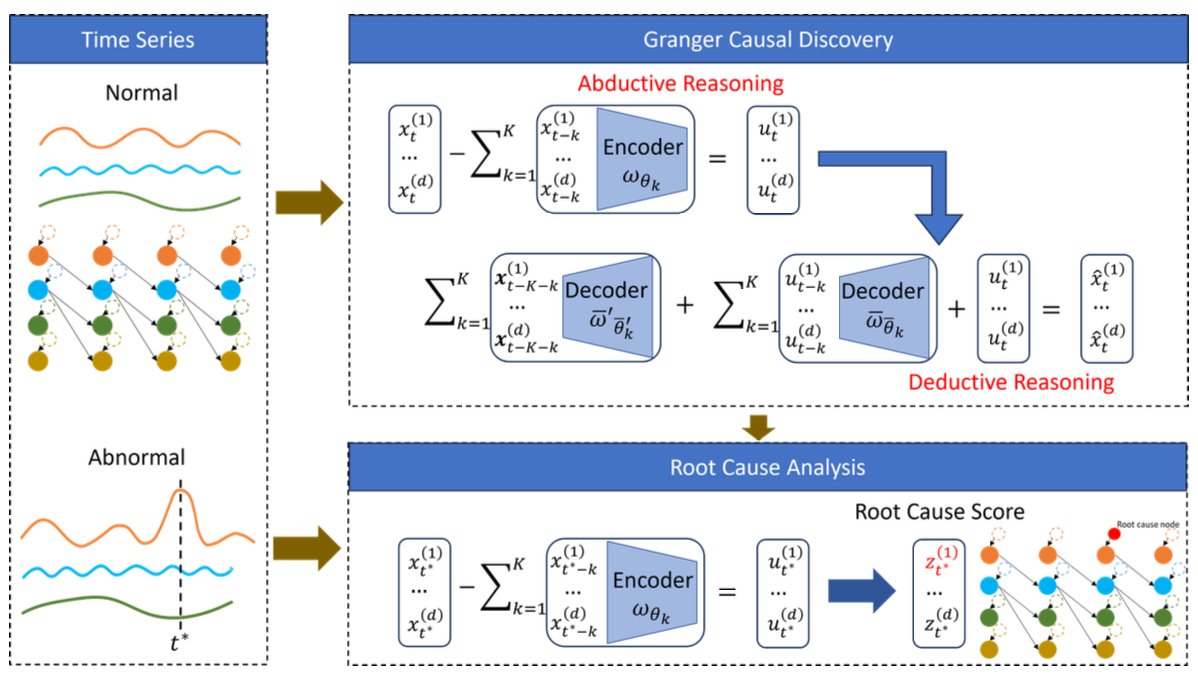
\includegraphics[width=0.9\textwidth]{figures/aerca.png}
  \caption{Minh họa cấu trúc AERCA dùng autoencoder để học phụ thuộc Granger trên chuỗi thời gian đa biến. Nguồn: Han và cộng sự \cite{han2025aerca}.}
  \label{fig:aerca-architecture}
\end{figure}

Trong CausClass, AERCA được dùng theo hai vai trò. Thứ nhất, mô hình tạo đồ thị khởi tạo và tín hiệu hệ số thô từ chuỗi hành vi. Thứ hai, AERCA có mask được dùng như bộ kiểm chứng cho các đồ thị ứng viên. Khi áp một mask cấu trúc, mô hình chỉ được phép sử dụng các liên kết nằm trong đồ thị ứng viên, từ đó đánh giá xem cấu trúc đó có đủ khả năng dự báo chuỗi \(X\) hay không.

Để tránh đồ thị quá dày, CausClass dùng điểm số kết hợp lỗi dự báo với phạt độ phức tạp. Một dạng tổng quát của điểm số là
\begin{equation}
\label{eq:graph-score}
    \mathcal{S}(G) = \mathcal{L}(X;G) + \lambda |E|,
\end{equation}
trong đó \(\mathcal{L}(X;G)\) là lỗi dự báo hoặc lỗi tái tạo khi mô hình bị ràng buộc bởi cấu trúc \(G\), \(|E|\) là số cạnh liên hành vi và \(\lambda\) là hệ số phạt độ phức tạp. Điểm số thấp hơn biểu thị ứng viên tốt hơn. Nguyên tắc này giúp đồ thị cuối cùng không chỉ khớp dữ liệu, mà còn đủ gọn để người dùng có thể kiểm tra và diễn giải.

Khi áp dụng vào dữ liệu lớp học, ba mức diễn giải cần được phân biệt rõ: tương quan đồng thời, liên kết dự báo theo thời gian và quan hệ nhân quả. Theo nền tảng suy luận nhân quả, diễn giải nhân quả đòi hỏi mô hình giả định và điều kiện nhận dạng mạnh hơn so với việc phát hiện phụ thuộc thống kê \,\cite{pearl2009causality,peters2017elements}. Dữ liệu video thụ động không có can thiệp và thường thiếu nhiều biến nền, nên đồ án chỉ sử dụng mức liên kết dự báo. Đây là lựa chọn thận trọng: đồ thị giúp người dùng xác định quan hệ thời gian đáng kiểm tra, còn kết luận sư phạm vẫn cần con người xem lại video và đặt kết quả vào bối cảnh lớp học.